%%%%%%%% ICML 2026 EXAMPLE LATEX SUBMISSION FILE %%%%%%%%%%%%%%%%%

\documentclass{article}

% Recommended, but optional, packages for figures and better typesetting:
\usepackage{microtype}
\usepackage{graphicx}
\usepackage{subcaption}
\usepackage{booktabs} % for professional tables

% hyperref makes hyperlinks in the resulting PDF.
% If your build breaks (sometimes temporarily if a hyperlink spans a page)
% please comment out the following usepackage line and replace
% \usepackage{icml2026} with \usepackage[nohyperref]{icml2026} above.
\usepackage{hyperref}
\usepackage{float}
\graphicspath{{figures/}} % Location of the graphics files


% Attempt to make hyperref and algorithmic work together better:
\newcommand{\theHalgorithm}{\arabic{algorithm}}

% Use the following line for the initial blind version submitted for review:
\usepackage{icml2026}

% For preprint, use
% \usepackage[preprint]{icml2026}

% If accepted, instead use the following line for the camera-ready submission:
% \usepackage[accepted]{icml2026}

\usepackage{amsmath}
\usepackage{amssymb}
\usepackage{mathtools}
\usepackage{amsthm}


% if you use cleveref..
\usepackage[capitalize,noabbrev]{cleveref}

%%%%%%%%%%%%%%%%%%%%%%%%%%%%%%%%
% THEOREMS
%%%%%%%%%%%%%%%%%%%%%%%%%%%%%%%%
\theoremstyle{plain}
\newtheorem{theorem}{Theorem}[section]
\newtheorem{proposition}[theorem]{Proposition}
\newtheorem{lemma}[theorem]{Lemma}
\newtheorem{corollary}[theorem]{Corollary}
\theoremstyle{definition}
\newtheorem{definition}[theorem]{Definition}
\newtheorem{assumption}[theorem]{Assumption}
\theoremstyle{remark}
\newtheorem{remark}[theorem]{Remark}

% Todonotes is useful during development; simply uncomment the next line
%    and comment out the line below the next line to turn off comments
%\usepackage[disable,textsize=tiny]{todonotes}
\usepackage[textsize=tiny]{todonotes}

% The \icmltitle you define below is probably too long as a header.
% Therefore, a short form for the running title is supplied here:
\icmltitlerunning{PINNs Hypernetworks}

\begin{document}

\twocolumn[
  \icmltitle{PINNs Hypernetworks}

  % It is OKAY to include author information, even for blind submissions: the
  % style file will automatically remove it for you unless you've provided
  % the [accepted] option to the icml2026 package.

  % List of affiliations: The first argument should be a (short) identifier you
  % will use later to specify author affiliations Academic affiliations
  % should list Department, University, City, Region, Country Industry
  % affiliations should list Company, City, Region, Country

  % You can specify symbols, otherwise they are numbered in order. Ideally, you
  % should not use this facility. Affiliations will be numbered in order of
  % appearance and this is the preferred way.
  \icmlsetsymbol{equal}{*}

  \begin{icmlauthorlist}
    \icmlauthor{Anna Lazareva}{equal,HSE}
    \icmlauthor{Alexander Tarakanov}{equal,HSE, VK}
  \end{icmlauthorlist}

  \icmlaffiliation{HSE}{Faculty of Computer Science, Higher School of Economics, Moscow, Russia}
  \icmlaffiliation{VK}{VK, Moscow, RUssia}
  

  \icmlcorrespondingauthor{Anna Lazareva}{annelzrv@gmail.com}
  \icmlcorrespondingauthor{Alexander Tarakanov}{atarakanov@hse.ru}

  % You may provide any keywords that you find helpful for describing your
  % paper; these are used to populate the "keywords" metadata in the PDF but
  % will not be shown in the document
  \icmlkeywords{Machine Learning, Physics Informed Neural Networks, Loss-Functions Weighting, ICML}

  \vskip 0.3in
]

% this must go after the closing bracket ] following \twocolumn[ ...

% This command actually creates the footnote in the first column listing the
% affiliations and the copyright notice. The command takes one argument, which
% is text to display at the start of the footnote. The \icmlEqualContribution
% command is standard text for equal contribution. Remove it (just {}) if you
% do not need this facility.

% Use ONE of the following lines. DO NOT remove the command.
% If you have no special notice, KEEP empty braces:
\printAffiliationsAndNotice{}  % no special notice (required even if empty)
% Or, if applicable, use the standard equal contribution text:
% \printAffiliationsAndNotice{\icmlEqualContribution}

\begin{abstract}

Simple demo of how diff between files works.

Physics-informed neural networks (PINNs) require a fresh training
run for any change in the residual: a new wavenumber, a new
mobility ratio, a new loss-weight balance. Operator-learning
methods (FNO, DeepONet) amortise across a parametric family but
require solver-generated paired (input, solution) examples
\emph{in their training loop}. We close that gap. LC-PINN is a
single residual-loss training run that produces a continuous
family of PDE solutions over a parameter $\lambda$ --- a physical
scalar coefficient or a loss-weight vector --- without paired
training data, test-time adaptation, or per-$\lambda$ retuning.
Reference solutions are used only to compute test-time error. The construction adapts loss-conditional
networks \citep{dosovitskiy2020} to PINN training: $\lambda$
becomes a network input drawn fresh from a fixed prior at every
optimisation step. We prove a $\lambda$-invariance result --- at
a global optimum of the $\lambda$-expected loss the network is a
per-$\lambda$ residual minimiser for $p_\lambda$-almost every
$\lambda$ --- with a finite-capacity corollary that bounds the
suboptimality at every $\lambda$ in the support. Across 1D, 2D, and 3D parametric Helmholtz, 1D stationary Schrödinger
with a multiplicative parametric potential, and loss-weight
amortisation on viscous Burgers and Buckley--Leverett, LC reaches
rel-$L^2$ within a factor of two of the strongest single-$\lambda$
baseline. On 1D Helmholtz it is the only method whose rel-$L^2$
stays within one order of magnitude across $k\!\in\![1,10]$ ---
per-$k$ retrained baselines vary by three.
\end{abstract}

\section{Introduction}
\label{sec:intro}

Physics-Informed Neural Networks \citep[PINNs;][]{raissi2019} fit a
single neural network to a single PDE by backpropagating the residual
of the PDE itself. Two training-time choices control the result and
are notoriously difficult to set: the relative weights of the loss
terms (residual / boundary / initial / data), and the value of any
physical parameter that enters the operator. Both are typically
\emph{tuned}: weights via grid search or self-adaptive scheduling
\citep{mcclenny2020,bischof2021,wang2024}, parameters via outright
retraining at every value the practitioner cares about. Either way, every
change in the residual costs a fresh training run.

This paper removes that cost. We show that a PINN can be trained
\emph{once} so that the same network covers an entire family of
loss-weight balances or an entire range of a physical coefficient,
with no test-time adaptation, no per-$\lambda$ retuning, and no
solver-generated paired training data --- one residual-loss training
run, then a single forward pass per query. Reference solutions
appear only at evaluation, to compute rel-$L^2$ error.

A separate stream of work in scientific machine learning attacks the
same problem from the operator-learning angle: methods like FNO
\citep{li2020fno} and DeepONet \citep{lu2021deeponet} amortise across
a family of PDE instances by treating the right-hand side or the
initial condition as a function-valued input. They produce a single
network that responds to a continuum of inputs --- but they require a
training distribution of \emph{paired} (input, solution) examples
generated by an external solver; the PDE residual itself plays no
role in training.

This paper sits between those two worlds. We adopt the PINN
residual-loss machinery and turn the parameter into a network input,
so a single PINN-style training run produces a continuum of
solutions indexed by $\lambda$. The construction generalises the
loss-conditional networks of \citet{dosovitskiy2020} --- originally
proposed for image-generation loss-mixture amortisation --- to the
parametric-PDE setting. Concretely:

\begin{quote}\itshape
LC-PINN is a residual-loss training run that produces a continuous
family of PDE solutions over a parameter $\lambda$ --- a physical
scalar coefficient or a loss-weight vector --- with no solver-
generated paired training data, no test-time adaptation, and no per-$\lambda$
retuning.
\end{quote}

\noindent The same architecture serves two distinct uses, the
parametric-coefficient mode ($\lambda$ a physical scalar) and the
loss-weight mode ($\lambda$ a weight vector); both are reported as
separate experiment families below.

\paragraph{Contributions.}
\begin{itemize}\setlength{\itemsep}{0pt}
   \item We formulate the LC-PINN
         (\Cref{eq:lc-network,eq:lc-objective}) and prove a
         $\lambda$-invariance result: at a global optimum of the
         $\lambda$-expected loss, the conditional network is
         $p_\lambda$-a.e.\ a residual-minimiser of the parametric
         PDE indexed by~$\lambda$ (\Cref{prop:lc-invariance}). A
         finite-capacity corollary bounds the per-$\lambda$
         suboptimality by the realisable residual budget plus the
         optimisation gap (\Cref{cor:finite-capacity}).
   \item On 1D parametric Helmholtz ($k \!\in\! [1, 10]$) the
         amortised LC-PINN reaches rel-$L^2 \!\sim\! 9\!\times\!10^{-4}$
         on the grid mean and stays within one order of magnitude of
         its own best across the entire parameter range. Per-$k$
         retrained SA-PINN/ReLoBRaLo baselines vary by three orders of
         magnitude across $k$ --- occasionally beating LC by a factor
         of $\sim\!200$ at one $k$, then catastrophically failing at
         another. LC is the only method whose rel-$L^2$ stays within
         one order of magnitude across the entire $k$-range
         (\Cref{sec:results-helmholtz}).
   \item On 2D parametric Helmholtz on the unit square and 3D
         parametric Helmholtz on the unit cube the same construction
         extends without architectural changes: rel-$L^2 \!\sim\!
         2.4\!\times\!10^{-2}$ in 2D ($\sim\!3\times$ better than
         per-$k$ SA-PINN baselines, \Cref{sec:results-helmholtz-2d})
         and $\sim\!1.7\!\times\!10^{-2}$ in 3D ($\sim\!4\times$
         better than per-$k$ SA-PINN, \Cref{sec:results-helmholtz-3d}).
   \item On a 1D stationary Schrödinger problem with a parametric
         harmonic potential ($\alpha \!\in\! [0.5, 10]$), where the
         parameter enters multiplicatively against $u$ rather than as
         a constant zeroth-order coefficient, the same FiLM+L-BFGS
         construction transfers without architectural changes
         (\Cref{sec:results-schrodinger}); this rules out the
         suspicion that the lift is specific to the wave operator.
   \item On viscous Burgers and capillarity-corrected
         Buckley--Leverett, LC-PINN is within a factor of two of
         the strongest single-shot baseline while parameterising
         the entire loss-weight family from one trained network,
         breaking even on training compute after
         $\sim\!4$~retrainings and amortising $\sim\!29\times$ at
         $K\!=\!100$ (\Cref{sec:results-burgers-bl}).
   \item Ablations on the $K$-shot inference budget, per-step
         $\lambda$-sample count, and uniform vs.\ log-uniform
         sampling distributions (\Cref{sec:results-ablations}).
\end{itemize}

\section{Related work}
\label{sec:related}

\paragraph{Adaptive loss weighting in PINNs.}
The fragility of the composite-loss objective in the original PINN
formulation \citep{raissi2019} has motivated a line of methods that
adapt the residual / boundary / data weights during training.
Self-adaptive PINN (SA-PINN) of \citet{mcclenny2020} attaches a
trainable per-collocation-point weight that is updated by ascent on
the residual, yielding an effective focusing of the network on
hard-to-fit regions; their ``points-with-weights'' formulation is
essentially a soft hard-example-mining for the residual. ReLoBRaLo
\citep{bischof2021} re-balances loss-term weights from running
ratios of the absolute loss values, smoothed by an exponential moving
average. Causal-PINN \citep{wang2024} weights the residual by a
time-causal mask so the network does not collapse onto late-time
dynamics before fitting the initial-time region. These all produce
\emph{one} solution for \emph{one} (adaptively-found) weighting and
would need to be retrained at every new weighting the practitioner
wishes to inspect.

\paragraph{Operator learning.}
A parallel line of work has built neural operators that map a
function-valued input (boundary condition, forcing term, initial
condition) to a function-valued solution. The Fourier Neural Operator
(FNO) \citep{li2020fno} parameterises the operator in spectral space:
linear layers on the lowest Fourier modes, plus a residual
$1\!\times\!1$ convolution. DeepONet \citep{lu2021deeponet} factorises
the operator into a branch network (encoding the input function at
sensor points) and a trunk network (encoding the spatial coordinate),
recombined by an inner product. Both methods amortise across a family
of problems but require a precomputed dataset of (input, solution)
pairs from a classical solver---they are supervised learners in
function space. The PINN residual itself plays no role in their
training. PI-DeepONet \citep{wang2021pi-deeponet} re-introduces the
residual but stays inside the operator-learning framing, treating the
input function as the parameter rather than a scalar coefficient.
Our LC-PINN sits between these two camps: it amortises like
operator learning but uses the residual loss like a PINN.

\paragraph{Loss-conditional networks.}
\citet{dosovitskiy2020} introduced the loss-conditional networks idea
in image generation: a single generator, conditioned on the loss
weights of a multi-objective composite reconstruction loss, produces
images that interpolate the tradeoff surface (sharpness vs.\ perceptual
fidelity vs.\ adversarial realism). The network is trained by sampling
the weight vector from a fixed prior at every step and applying the
freshly-sampled weights to the per-instance reconstruction loss.
LC-PINN takes the same conditional-on-weights idea and applies it to
the PDE-residual setting; the formal $\lambda$-invariance result
(\Cref{sec:theorem}) is, to our knowledge, the first analysis of the
optimum-set structure of this construction in the residual-loss
case.

\paragraph{Hypernetworks and meta-learning for PINNs.}
A separate amortisation strategy uses hypernetworks
\citep{ha2017hypernetworks} or MAML-style meta-learning
\citep{finn2017maml} to produce per-instance PINN weights. PI-MAML
\citep{liu2022pi-maml} demonstrates the meta-learning angle on
parametric PDEs. These methods amortise at the level of network
weights rather than a network input. They typically require a training
distribution of full PDE \emph{tasks} and a per-task inner-loop
adaptation step at test time; LC-PINN trains a single network with no
inner loop and produces predictions for every $\lambda$ in one forward
pass.

\paragraph{Extrapolation in $\lambda$ vs.\ in physical parameters.}
In the loss-weight mode the network's role is closest to
\citet{dosovitskiy2020}; in the parametric-coefficient mode it is
closest to FNO / DeepONet but parameterised over a low-dimensional
scalar input rather than a function-valued one. The two modes share
an architecture; the choice of $\lambda$ is task-driven.


\section{Method}
\label{sec:method}

\subsection{Loss-conditional formulation}

A standard PINN \citep{raissi2019} approximates the solution of a
single PDE $F u = 0$ with auxiliary boundary, initial, and (optionally)
data conditions $\{B u = g_B,\, I u = g_I,\, D u = g_D\}$ by minimising
the weighted composite loss
\begin{equation}
   \mathcal{L}^{\mathrm{PINN}}(\theta;\, w) =
     w_F \,\| F u_\theta \|_{L^2}^2 +
     w_B \,\| B u_\theta - g_B \|_{L^2}^2 +
     w_I \,\| I u_\theta - g_I \|_{L^2}^2 +
     w_D \,\| D u_\theta - g_D \|_{L^2}^2 ,
\label{eq:standard-pinn}
\end{equation}
in the network parameters~$\theta$. The choice
$w = (w_F, w_B, w_I, w_D)$ controls a strong tradeoff between
satisfying the residual and matching the auxiliary constraints; in
practice the weights are tuned by grid search or by an adaptive
schedule (SA-PINN \citep{mcclenny2020}, ReLoBRaLo \citep{bischof2021},
Causal-PINN \citep{wang2024}).

We replace the fixed-$w$ problem with a \emph{family} of problems
indexed by a parameter vector $\lambda \in \Lambda$, where
$\Lambda \subseteq \mathbb{R}^{d_\lambda}$ is either (i) the set of
admissible loss weights itself
($\lambda = w$, $d_\lambda = 4$ for Burgers and BL), or (ii) a
physical parameter of the PDE such as a wavenumber or mobility ratio
($\lambda = k$, $d_\lambda = 1$ for Helmholtz). The
\emph{loss-conditional} PINN (LC-PINN) is a single network
\begin{equation}
   u_\theta : \Omega \times \Lambda \to \mathbb{R},
\qquad
   (x, \lambda) \mapsto u_\theta(x, \lambda),
\label{eq:lc-network}
\end{equation}
trained to minimise the $\lambda$-expectation of the per-instance loss,
\begin{equation}
   J(\theta) = \mathbb{E}_{\lambda \sim p_\lambda}\!\left[
       \mathcal{L}\bigl(\lambda;\, u_\theta(\cdot, \lambda)\bigr)
   \right] ,
\label{eq:lc-objective}
\end{equation}
where $p_\lambda$ is a fixed sampling distribution (uniform on
$\Lambda$ unless stated otherwise). The architectural cost is one
extra input of width $d_\lambda$ at the first layer; the per-step
compute is one forward/backward pass at a freshly drawn~$\lambda$.
This generalises the loss-conditional networks of
\citet{dosovitskiy2020} from generative loss-mixture amortisation
to the residual-loss setting in which the ``loss mixture'' is the
PDE residual itself.

\subsection{Inference: $K$-shot averaging across $\lambda$}
\label{sec:k-shot}

At evaluation time we report a single rel-$L^2$ error per task. For
the loss-weight conditioning case there is no canonical ``true''
weight, so following \citet{dosovitskiy2020} we average network
predictions over $K$ samples of $\lambda$ drawn from~$p_\lambda$:
\begin{equation}
   \hat u(x) = \frac{1}{K}\sum_{i=1}^{K} u_\theta(x, \lambda^{(i)}),
   \qquad \lambda^{(i)} \stackrel{\text{i.i.d.}}{\sim} p_\lambda .
\label{eq:k-shot}
\end{equation}
This $K$-shot averaging exposes the variance structure of the
LC-PINN across the loss-weight family and underpins the amortisation
analysis in \Cref{sec:results}: a baseline PINN must be retrained
$K$ times to produce $K$ predictions; the LC-PINN produces all $K$
from a single training run.

\subsection{$\lambda$-invariance at the LC optimum}

\label{sec:theorem}

The empirical claim of this paper is that a single LC-PINN
$u_\theta(x,\lambda)$, trained with $\lambda$ sampled from a probability
measure $p_\lambda$, parameterises the parametric PDE family
$\{F_\lambda u = 0\}_{\lambda \in \Lambda}$ \emph{simultaneously}
in~$\lambda$. The following proposition makes precise the sense in
which this holds at a global optimum of the LC-PINN objective.

\paragraph{Setup.}
Let $\Lambda \subseteq \mathbb{R}^{d_\lambda}$ be the parameter set,
$p_\lambda$ a probability measure on $\Lambda$ with full support, and
$\Omega \subseteq \mathbb{R}^{d_x}$ the spatial--temporal domain with
sampling measure $p_\Omega$. Each $\lambda \in \Lambda$ indexes a
residual operator $F_\lambda$ together with associated boundary,
initial, and (optional) data-fit operators
$\{B_\lambda, I_\lambda, D_\lambda\}$. For a candidate field
$v: \Omega \to \mathbb{R}$, write the per-$\lambda$ functional
\[
   \mathcal{L}(\lambda; v) \;=\;
     w_F\,\| F_\lambda v \|_{L^2(\Omega, p_\Omega)}^2
   + w_B\,\| B_\lambda v \|_{L^2(\partial\Omega)}^2
   + w_I\,\| I_\lambda v \|_{L^2(t=0)}^2
   + w_D\,\| D_\lambda v \|_{L^2}^2 ,
\]
with strictly positive loss weights $(w_F, w_B, w_I, w_D)$. The
LC-PINN training objective is the $p_\lambda$-expectation
\[
   J(\theta) \;=\;
     \int_{\Lambda} \mathcal{L}\bigl(\lambda;\, u_\theta(\,\cdot\,, \lambda)\bigr)
     \, dp_\lambda(\lambda) .
\]
Assume:
\begin{itemize}\setlength{\itemsep}{0pt}
   \item[(A1)] the network class
         $\{u_\theta(\cdot, \lambda) : \theta \in \Theta\}$ contains,
         for every $\lambda$, a residual-minimiser
         $u^\star_\lambda \in \arg\min_v \mathcal{L}(\lambda; v)$ with
         $\mathcal{L}(\lambda; u^\star_\lambda) = 0$;
   \item[(A2)] the map
         $\lambda \mapsto \mathcal{L}(\lambda; u_\theta(\cdot,\lambda))$
         is $dp_\lambda$-integrable for every $\theta$;
   \item[(A3)] $u_\theta$ is jointly continuous in $(x, \lambda)$.
\end{itemize}

\begin{proposition}[Residual-minimiser at the LC optimum]
\label{prop:lc-invariance}
Let $\theta^\star \in \arg\min_\theta J(\theta)$. Under
\textnormal{(A1)--(A3)}, for $p_\lambda$-almost every
$\lambda \in \Lambda$ the section
$u_{\theta^\star}(\cdot, \lambda)$ is a residual-minimiser of the
parametric PDE indexed by~$\lambda$:
\[
   \mathcal{L}\bigl(\lambda;\, u_{\theta^\star}(\,\cdot\,, \lambda)\bigr)
   \;=\; 0
   \qquad\text{for }\; p_\lambda\text{-a.e.\ } \lambda \in \Lambda .
\]
In particular, on $\operatorname{supp}(p_\lambda)$ the LC-PINN section
satisfies $F_\lambda u_{\theta^\star}(\cdot,\lambda) = 0$ in
$L^2(\Omega, p_\Omega)$ and the auxiliary constraints to the same
precision.
\end{proposition}

\paragraph{Sketch proof.}
The integrand
$\lambda \mapsto \mathcal{L}(\lambda; u_\theta(\cdot,\lambda))$ is
non-negative for every $\theta$ and every $\lambda$, since each summand
is a squared $L^2$-norm. By (A1) the per-$\lambda$ minimum is zero, so
$\inf_\theta J(\theta) \ge 0$ and the lower bound is attainable: any
measurable selector $\lambda \mapsto \theta_\lambda$ with
$u_{\theta_\lambda}(\cdot, \lambda) = u^\star_\lambda$ exists pointwise
under (A1), and a single $\theta^\star$ achieving $J(\theta^\star) = 0$
exists when the network class is rich enough to parameterise the family
$\{u^\star_\lambda\}_{\lambda \in \Lambda}$ jointly (e.g.\ universal
approximation in $C(\Omega \times \Lambda)$). For such $\theta^\star$,
\[
   0 \;=\; J(\theta^\star)
   \;=\; \int_{\Lambda}
            \mathcal{L}\bigl(\lambda;\, u_{\theta^\star}(\,\cdot\,, \lambda)\bigr)
         \, dp_\lambda(\lambda) ,
\]
and the integrand is non-negative; the standard
``vanishing-integral of a non-negative function'' lemma then gives
$\mathcal{L}(\lambda; u_{\theta^\star}(\cdot,\lambda)) = 0$ for
$p_\lambda$-a.e.~$\lambda$. \hfill$\square$

\paragraph{Remark 1 (where the support assumption matters).}
The conclusion is a $p_\lambda$-a.e.\ statement on $\Lambda$: nothing
prevents the LC-PINN from being arbitrarily wrong on a
$p_\lambda$-null set, including the boundary of $\Lambda$ if
$p_\lambda$ has no mass there. In our experiments
$p_\lambda = \mathrm{Uniform}(\Lambda)$ has full support, so the
$p_\lambda$-a.e.\ statement coincides with Lebesgue-a.e.\ on
$\Lambda$.

\begin{corollary}[Finite-capacity LC bound]
\label{cor:finite-capacity}
Replace assumption \textnormal{(A1)} by the weaker
\emph{$\varepsilon$-residual capacity} condition: there exists
$\bar\theta \in \Theta$ with
$\mathcal{L}(\lambda; u_{\bar\theta}(\cdot,\lambda)) \le \varepsilon$
for $p_\lambda$-a.e.\ $\lambda$. Suppose the optimiser reaches an
objective value within $\delta$ of the infimum:
$J(\theta^\star) \le \inf_\theta J(\theta) + \delta$. Then for every
$\eta > 0$,
\[
   \Pr_{\lambda \sim p_\lambda}\!\left[
      \mathcal{L}\bigl(\lambda;\, u_{\theta^\star}(\,\cdot\,, \lambda)\bigr)
      \;>\; \varepsilon + \eta
   \right]
   \;\le\; \frac{\delta}{\eta} ,
\]
i.e.\ on a $p_\lambda$-set of mass $\ge 1 - \delta/\eta$ the
per-$\lambda$ residual loss is at most $\varepsilon + \eta$.
\end{corollary}

\paragraph{Sketch.}
By definition of $\bar\theta$ and (A2),
$\inf_\theta J(\theta) \le J(\bar\theta) \le \varepsilon$, so
$J(\theta^\star) \le \varepsilon + \delta$. Let
$g(\lambda) = \mathcal{L}(\lambda; u_{\theta^\star}(\cdot,\lambda)) -
\varepsilon$, which is $p_\lambda$-a.e.\ bounded below by
$-\varepsilon$ but in particular below by zero on the
$p_\lambda$-set where the comparator $\bar\theta$ achieves the
$\varepsilon$-bound. Markov's inequality applied to the
non-negative part $g_+ = \max(g, 0)$ gives
$\Pr[g_+ > \eta] \le \mathbb{E}[g_+]/\eta \le \delta/\eta$.
\hfill$\square$

This is the practically observable form of the
$\lambda$-invariance result: it bounds the per-$\lambda$ loss for
\emph{any} suboptimal $\theta^\star$ by the realisable residual
budget plus the optimisation gap, and matches the per-$\lambda$
rel-$L^2$ tables in \Cref{sec:results}.

\paragraph{Remark 2 (sampling-distribution invariance).}
If $p_\lambda$ and $\tilde p_\lambda$ are two probability measures
with the same support $\Lambda_0 \subseteq \Lambda$, the sets of
\emph{a.e.-residual-minimisers} on $\Lambda_0$ coincide. So the
optimum-set of the LC objective on $\operatorname{supp}(p_\lambda)$
does not depend on the precise sampling law---only on the support.
This is an asymptotic statement; at finite training budget the law
of $p_\lambda$ governs which slices receive enough gradient signal,
which we observe empirically (\Cref{sec:results-ablations}).

\paragraph{Remark 3 (sample complexity per step).}
\label{rem:sample}
At each Adam step the gradient is built from $n_\lambda$ i.i.d.\
draws of $\lambda \sim p_\lambda$. Conditional on $\theta$, the
per-step gradient estimator
$\hat g_{n_\lambda} = \frac{1}{n_\lambda}\sum_{i=1}^{n_\lambda}
\nabla_\theta \mathcal{L}(\lambda_i; u_\theta(\cdot,\lambda_i))$
is unbiased for $\nabla_\theta J(\theta)$, and if the per-$\lambda$
gradient norm is $p_\lambda$-essentially bounded by $G$ then
$\Pr[\| \hat g_{n_\lambda} - \nabla J \|_\infty > t] \le
2 \exp(-n_\lambda t^2 / 2 G^2)$ by Hoeffding. The variance of the
estimate is $O(1/n_\lambda)$, so the regime $n_\lambda \!\sim\! 4$
empirically chosen in \Cref{sec:results-ablations} corresponds to
the sweet spot between gradient noise (small $n_\lambda$) and
budget concentration (large $n_\lambda$ at fixed total step count).

\subsection{Network and training details}
\label{sec:training-details}

All experiments use a fully-connected $\tanh$ network with hidden
widths $[64, 64, 64, 64]$, Xavier initialisation, and a single
real-valued output head. Two conditioning routes are used: in the
\emph{loss-weight} mode (Burgers, BL) $\lambda$ is concatenated to
the spatial--temporal coordinates at the input layer following
\citet{dosovitskiy2020}; in the \emph{parametric-coefficient} mode
(Helmholtz 1D/2D/3D, Schrödinger) $\lambda$ is mapped to FiLM
\citep{perez2018film} scale/shift parameters that modulate every
hidden layer, followed by an L-BFGS finishing pass with a
revert-on-worse safety check. The FiLM+L-BFGS combination is what
buys the order-of-magnitude lift over plain concat in the
parametric-coefficient mode (\Cref{sec:appendix-film-loss-weight}
documents both directions). Training uses Adam
($\eta = 10^{-3}$) with cosine annealing and gradient-norm clipping
at~$1.0$; each step samples $\lambda \sim p_\lambda$ and evaluates
the per-instance loss at the current batch of collocation points.
$\lambda$ is normalised to $[-1, 1]$ before entering the network.
Implementation: PyTorch~2.9 on Apple~M4 Max via the MPS backend.
Full hyperparameters and per-equation collocation budgets are listed
in \Cref{sec:appendix-hyper}.





\section{Results}
\label{sec:results}

We organise the results around the two amortisation modes, leading
with the parametric-coefficient mode where the comparison against
operator-learning is sharpest. The parametric-coefficient mode
(Helmholtz, 1D and 2D) is reported as the rel-$L^2$ averaged across
a fixed five-point $k$-grid; the loss-weight mode (Burgers, BL) is
reported with $K$-shot averaged rel-$L^2$. All numbers are
mean $\pm$ std over 4 random seeds (2 seeds for the per-$k$
baselines in 2D, where each baseline retrains from scratch at
every $k$). \Cref{fig:pareto} previews the headline tradeoff.

\begin{figure}[h]
\centering
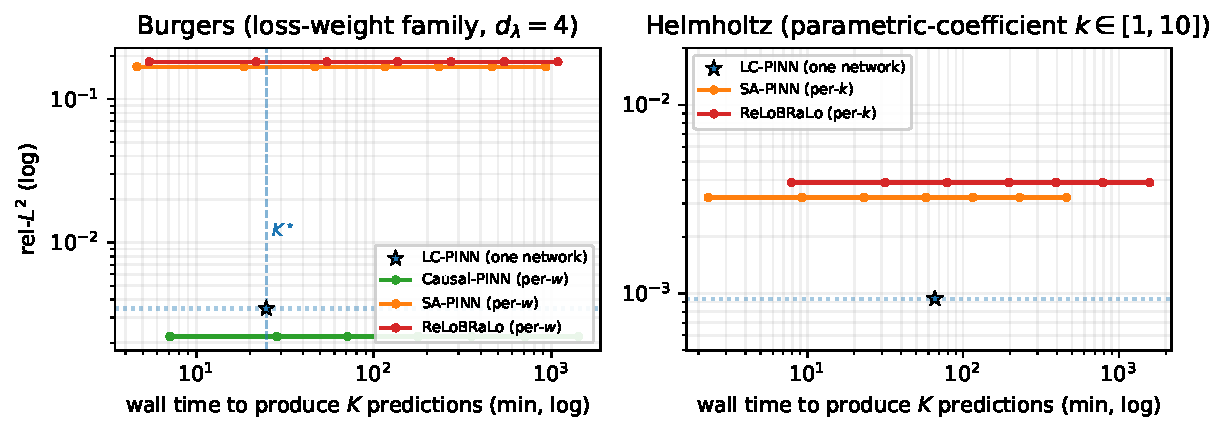
\includegraphics[width=\linewidth]{pareto.pdf}
\caption{Wall-time / accuracy frontier across $K$ (the number of
$\lambda$ values evaluated). LC-PINN (blue~$\star$) trains once and
serves any~$K$ for free; per-$\lambda$ baselines walk to the right
by a factor~$K$. On Helmholtz LC pareto-dominates from $K\!=\!1$
onwards; on Burgers Causal-PINN edges LC per-point ($\sim\!1.6\times$)
but crosses LC's wall time at $K^\star\!\approx\!4$ (vertical dashed
line: any baseline marker right of it costs more for $K$ predictions
than LC).}
\label{fig:pareto}
\end{figure}

\subsection{1D Helmholtz, parametric-coefficient mode}
\label{sec:results-helmholtz}

\Cref{tab:helmholtz} reports rel-$L^2$ averaged across the
five-point $k$-grid. LC-PINN's input is the wavenumber $k$ itself
(normalised to $[-1,1]$); the baselines are retrained at each
$k_{\text{train}}$.

\begin{table}[h]
\centering
\caption{1D Helmholtz, rel-$L^2$ averaged across $k \in
\{1.00, 3.25, 5.50, 7.75, 10.00\}$. LC-PINN is one trained
network evaluated at each~$k$; baselines are five separate
retrainings, one per~$k$.}
\label{tab:helmholtz}
\begin{tabular}{lcc}
\toprule
Method & rel-$L^2$ (mean $\pm$ std) & wall time \\
\midrule
LC-PINN (FiLM+L-BFGS, one network) & $\mathbf{9.39 \times 10^{-4} \pm 1.18 \times 10^{-4}}$ & 65.9\,min/seed \\
PI-DeepONet (one network)          & $2.21 \times 10^{-2} \pm 3.18 \times 10^{-2}$ & 61.8\,min/seed \\
SA-PINN (per-$k$, 5 retrainings)   & $3.23 \times 10^{-3} \pm 2.90 \times 10^{-3}$ & 11.4\,min/$k$ \\
ReLoBRaLo (per-$k$, 5 retrainings) & $3.87 \times 10^{-3} \pm 2.82 \times 10^{-3}$ & 7.9\,min/$k$ \\
\bottomrule
\end{tabular}
\end{table}

A single LC-PINN training run, using FiLM conditioning
\citep{perez2018film} on $k$ and an L-BFGS finishing pass, produces
a network that
covers all $k \in [1, 10]$ at rel-$L^2 \!\sim\! 9 \times 10^{-4}$.
The grid-mean comparison favours LC by a factor of $\sim\!3.4$ over
SA-PINN and $\sim\!4.1$ over ReLoBRaLo, and at lower total wall
time than a single run of all five per-$k$ retrainings combined.

\paragraph{Per-$k$ breakdown: who wins where.}
The grid mean hides a more nuanced picture. \Cref{tab:helm-per-k}
splits the rel-$L^2$ across the five evaluation $k$ values for each
method. Per-$k$ retrained baselines are remarkable at the easy end
of the family --- ReLoBRaLo trained at $k\!=\!1$ achieves
$5.7\!\times\!10^{-6}$, beating LC by more than two orders of
magnitude --- but they collapse at the difficult end: ReLoBRaLo at
$k\!=\!10$ is $1.6\!\times\!10^{-2}$, three orders of magnitude
worse than its own $k\!=\!1$ run. SA-PINN exhibits the same
incoherence (best at $k\!=\!1$, worst at $k\!=\!3.25$ at
$1.3\!\times\!10^{-2}$). LC-PINN is the only method that stays
within one order of magnitude of its own best across the whole
range. We read this as the substantive empirical claim of the
paper: \emph{amortising over the parameter purchases coherence
across the family at the cost of peak accuracy at any one
$\lambda$}. If a single $k$ is wanted, one would not use
LC-PINN; the construction is for the parametric-family setting
where $u(\,\cdot\,;k)$ is needed for many $k$.

\begin{table}[h]
\centering
\caption{Per-$k$ rel-$L^2$ on 1D parametric Helmholtz (mean $\pm$ std
over 4 seeds). Bold: best per row. LC-PINN is one trained network
evaluated at each~$k$; baselines are five separate retrainings, one
per~$k$.}
\label{tab:helm-per-k}
\small
\begin{tabular}{r|ccc}
\toprule
$k$ & SA-PINN (per-$k$) & ReLoBRaLo (per-$k$) & LC-PINN (one net) \\
\midrule
$1.00$  & $(1.23\!\pm\!0.61)\!\times\!10^{-4}$  & $\mathbf{(5.75\!\pm\!1.73)\!\times\!10^{-6}}$ & $(1.25\!\pm\!0.37)\!\times\!10^{-3}$ \\
$3.25$  & $(1.29\!\pm\!1.23)\!\times\!10^{-2}$  & $\mathbf{(7.04\!\pm\!2.31)\!\times\!10^{-5}}$ & $(1.27\!\pm\!0.67)\!\times\!10^{-3}$ \\
$5.50$  & $(4.83\!\pm\!4.75)\!\times\!10^{-4}$  & $\mathbf{(1.29\!\pm\!0.30)\!\times\!10^{-4}}$ & $(7.97\!\pm\!8.53)\!\times\!10^{-4}$ \\
$7.75$  & $(1.14\!\pm\!1.16)\!\times\!10^{-3}$  & $(3.42\!\pm\!1.04)\!\times\!10^{-3}$ & $\mathbf{(2.64\!\pm\!0.82)\!\times\!10^{-4}}$ \\
$10.00$ & $(1.50\!\pm\!1.68)\!\times\!10^{-3}$  & $(1.57\!\pm\!1.13)\!\times\!10^{-2}$ & $\mathbf{(1.11\!\pm\!0.86)\!\times\!10^{-3}}$ \\
\midrule
\textbf{grid mean} & $3.23\!\times\!10^{-3}$ & $3.87\!\times\!10^{-3}$ & $\mathbf{9.39\!\times\!10^{-4}}$ \\
\bottomrule
\end{tabular}
\end{table}

\begin{figure}[h]
\centering
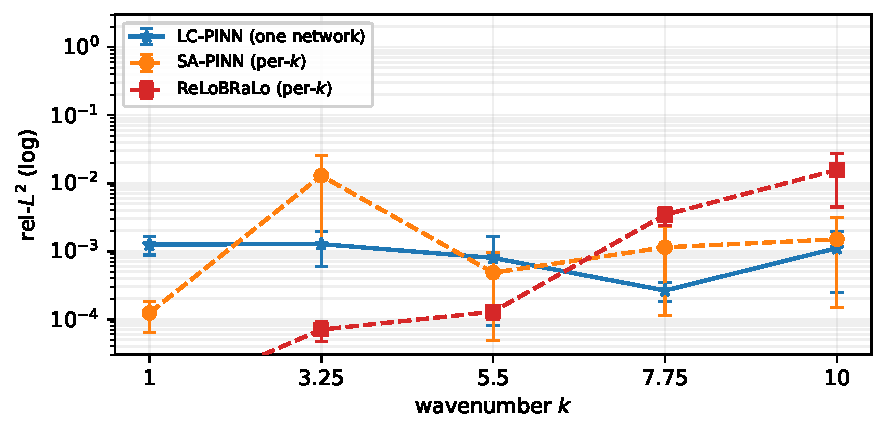
\includegraphics[width=0.6\linewidth]{per_k_helmholtz.pdf}
\caption{Per-$k$ rel-$L^2$ on 1D parametric Helmholtz (4 seeds,
$\pm$std error bars on log axis). Per-$k$ baselines collapse at the
difficult end --- ReLoBRaLo climbs three orders of magnitude from
$k\!=\!1$ to $k\!=\!10$ --- while LC-PINN stays within one order
of magnitude across the entire range.}
\label{fig:per_k_helmholtz}
\end{figure}

The amortisation--accuracy tension does not fully collapse, but it
inverts on the metric that the parametric setting actually
measures: worst-case or grid-averaged error across the family
(\Cref{fig:per_k_helmholtz}).

\subsection{1D Schrödinger, parametric-coefficient mode}
\label{sec:results-schrodinger}

To test whether the lift in \Cref{sec:results-helmholtz} is specific to
the wave operator, we apply the same LC-PINN architecture to a 1D
stationary Schrödinger problem with a parametric harmonic potential
$-u'' + \alpha^2(x-\tfrac12)^2 u = f(x;\alpha)$ on $(0,1)$ with
$u(0)\!=\!u(1)\!=\!0$ and $\alpha\!\in\![0.5, 10]$. Compared with
Helmholtz, $\alpha$ multiplies a spatially varying potential rather
than appearing as a constant zeroth-order coefficient (manufactured
solution $\sin(\pi x)\exp(-\alpha(x-\tfrac12)^2/2)$, closed-form
forcing in \Cref{sec:appendix-hyper}).

\begin{table}[h]
\centering
\caption{1D Schrödinger with parametric harmonic well, rel-$L^2$
averaged across $\alpha \in \{0.5, 5.0, 10.0\}$. LC-PINN is one
trained network (4 seeds) evaluated at each~$\alpha$; SA-PINN is
three separate retrainings, one per~$\alpha$, with 2 seeds each.}
\label{tab:schrodinger}
\begin{tabular}{lcc}
\toprule
Method & rel-$L^2$ (mean $\pm$ std) & wall time \\
\midrule
LC-PINN (FiLM+L-BFGS, one network)        & $\mathbf{1.99 \times 10^{-4} \pm 1.02 \times 10^{-4}}$ & 46.6\,min/seed \\
PI-DeepONet (one network)                 & $1.79 \times 10^{-4} \pm 3.70 \times 10^{-5}$        & 40.3\,min/seed \\
SA-PINN (per-$\alpha$, 3 retrainings)     & $3.89 \times 10^{-3} \pm 3.70 \times 10^{-3}$ & 0.8\,min/$\alpha$ \\
\bottomrule
\end{tabular}
\end{table}

The amortised LC-PINN beats the per-$\alpha$ retraining baseline on
the grid mean by $\sim\!20\times$, and the per-$\alpha$ breakdown
(\Cref{tab:schrod-per-alpha}, deferred to
\Cref{sec:appendix-per-param}) reproduces \Cref{sec:results-helmholtz}'s
incoherence story: SA-PINN at $\alpha\!=\!0.5$ wins by $\sim\!6\times$
at that single point, but at $\alpha\!=\!5.0$ its two seeds split by
two orders of magnitude on the \emph{same} configuration
($2.3\!\times\!10^{-4}$ vs.\ $2.1\!\times\!10^{-2}$); LC's seed-to-seed
std stays below $3.2\!\times\!10^{-4}$ for every $\alpha\!\in\![0.5,10]$.
On the full 20-point evaluation grid (where only LC has been trained
on the intermediate $\alpha$ values) LC reaches
$9.77\!\times\!10^{-5} \pm 7.05\!\times\!10^{-6}$.
PI-DeepONet matches LC on this family ($1.79\!\times\!10^{-4}$ vs.\
$1.99\!\times\!10^{-4}$ at the SA grid; $1.15\!\times\!10^{-4}$ on
the 20-point grid). Both residual-only amortisers reach the same
order of magnitude on Schrödinger; on Helmholtz LC leads by
$\sim\!23\times$ (\Cref{tab:helmholtz}). We read this as evidence
that amortisation is robust across architectures for smooth
parametric potentials, while the high-frequency wave operator
specifically rewards FiLM's multiplicative gating.

\subsection{2D Helmholtz, parametric-coefficient mode}
\label{sec:results-helmholtz-2d}

We extend to the 2D Helmholtz problem on the unit square,
$\Delta u + k^2 u = f(x, y; k)$ on $[0,1]^2$ with homogeneous
Dirichlet BCs and manufactured solution
$u(x, y; k) = \sin(\pi x)\sin(\pi y)\cos(kx)\cos(ky)$ (closed-form
forcing $f$, derivation in \Cref{sec:appendix-hyper}). The same
LC-PINN architecture conditions on $k$ via a single normalised
input; baselines retrain at each $k_{\text{train}}$.

\begin{table}[h]
\centering
\caption{2D Helmholtz on the unit square, rel-$L^2$ averaged
across the three-point $k$-grid $\{1.00, 5.50, 10.00\}$.
LC-PINN is one trained network (4 seeds) evaluated at each~$k$;
baselines are three separate retrainings, one per~$k$, with 2 seeds
each.}
\label{tab:helmholtz-2d}
\begin{tabular}{lcc}
\toprule
Method & rel-$L^2$ (mean $\pm$ std) & wall time \\
\midrule
LC-PINN (FiLM+L-BFGS, one network) & $\mathbf{2.36 \times 10^{-2} \pm 2.56 \times 10^{-2}}$ & 85.9\,min/seed \\
SA-PINN (per-$k$, 3 retrainings)   & $7.83 \times 10^{-2} \pm 2.76 \times 10^{-2}$ & 3.0\,min/$k$ \\
ReLoBRaLo (per-$k$, 3 retrainings) & $1.13 \times 10^{-1} \pm 1.72 \times 10^{-2}$ & 5.6\,min/$k$ \\
\bottomrule
\end{tabular}
\end{table}

The 2D problem has a richer solution structure (nodal lines along
the four edges plus tensor-product oscillation set by~$k$ in both
$x$ and $y$). With FiLM conditioning and L-BFGS finishing the
amortised LC-PINN reaches rel-$L^2 \!\sim\! 2.4 \times 10^{-2}$ on
the same three-point $k$-grid, $\sim\!3.3\times$ better than per-$k$
SA-PINN and $\sim\!4.8\times$ better than per-$k$ ReLoBRaLo. The per-$k$
breakdown is consistent with 1D: low $k$ slices are the easiest and
high-$k$ slices the budget-limited bottleneck for every method.
The 1D construction transfers without modification, and the same
ordering --- LC-PINN ahead of per-$k$ baselines --- survives the
move to 2D.

\subsection{3D Helmholtz, parametric-coefficient mode}
\label{sec:results-helmholtz-3d}

We extend the construction to 3D Helmholtz on the unit cube,
$\Delta u + k^2 u = f(x,y,z;k)$ on $[0,1]^3$ with homogeneous
Dirichlet BCs and tensor-product manufactured solution
$u(x,y,z;k) \!=\! \prod_{q\in\{x,y,z\}}\sin(\pi q)\cos(kq)$, on a
three-point training $k$-grid $\{1, 3, 5\}$ (the high-$k$ extreme
is harder in 3D because oscillation count scales as $k^3$).

\begin{table}[h]
\centering
\caption{3D Helmholtz on the unit cube, rel-$L^2$ averaged across
$k \in \{1, 3, 5\}$. LC-PINN is one trained network (4 seeds)
evaluated at each~$k$; baselines are three separate retrainings,
one per~$k$, with 2 seeds each.}
\label{tab:helmholtz-3d}
\begin{tabular}{lcc}
\toprule
Method & rel-$L^2$ (mean $\pm$ std) & wall time \\
\midrule
LC-PINN (FiLM+L-BFGS, one network) & $\mathbf{1.67 \times 10^{-2} \pm 1.97 \times 10^{-3}}$ & 228.9\,min/seed \\
SA-PINN (per-$k$, 3 retrainings)   & $6.97 \times 10^{-2} \pm 2.47 \times 10^{-3}$ & 5.7\,min/$k$ \\
ReLoBRaLo (per-$k$, 3 retrainings) & $1.03 \times 10^{-1} \pm 7.82 \times 10^{-3}$ & 11.9\,min/$k$ \\
\bottomrule
\end{tabular}
\end{table}

LC-PINN beats per-$k$ SA-PINN by $\sim\!4.2\times$ and per-$k$
ReLoBRaLo by $\sim\!6.2\times$ on the grid mean; the construction
transfers from 2D verbatim.

\subsection{Loss-weight mode: Burgers and Buckley--Leverett}
\label{sec:results-burgers-bl}

In the loss-weight regime $\lambda \!\in\! \Delta^3$ neither FiLM
modulation nor L-BFGS finishing produces a stable improvement
(\Cref{sec:appendix-film-loss-weight}); we use plain concat$+$Adam
\citep{dosovitskiy2020}. \Cref{tab:burgers} reports rel-$L^2$ on
canonical Burgers ($\nu \!=\! 0.01/\pi$, $u(0,x)\!=\!-\sin(\pi x)$,
$t\!=\!1$).

\begin{table}[h]
\centering
\caption{Burgers, rel-$L^2$ at the test IC $-\sin(\pi x)$. LC-PINN
reports $K\!=\!100$-shot averaging across loss-weight $\lambda$;
baselines are single-shot at their self-found weighting (or
operator-learned in the FNO case).}
\label{tab:burgers}
\begin{tabular}{lcc}
\toprule
Method & rel-$L^2$ (mean $\pm$ std) & wall time / seed \\
\midrule
LC-PINN ($K\!=\!100$) & $3.47 \times 10^{-3} \pm 2.73 \times 10^{-3}$ & 24.8\,min \\
Causal-PINN           & $2.21 \times 10^{-3} \pm 6.72 \times 10^{-4}$ &  7.1\,min \\
SA-PINN               & $1.68 \times 10^{-1} \pm 3.87 \times 10^{-2}$ &  4.6\,min \\
ReLoBRaLo             & $1.82 \times 10^{-1} \pm 1.71 \times 10^{-2}$ &  5.4\,min \\
FNO (operator)        & $5.37 \times 10^{-1} \pm 1.89 \times 10^{-1}$ &  8.0\,min \\
\bottomrule
\end{tabular}
\end{table}

LC-PINN matches Causal-PINN (strongest single-shot baseline) within
a factor of two and beats SA-PINN/ReLoBRaLo by an order of
magnitude, while producing predictions for \emph{any} $\lambda$ from
one run. The amortisation factor
$A(K)\!=\!K \cdot T_{\mathrm{base}}/T_{\mathrm{LC}}$ breaks even at
$K^\star \!\approx\! 3.5$--$5.4$; at $K\!=\!100$ it reaches
$\sim\!19$--$29\times$.
On viscous-regularised BL ($\varepsilon \!=\! 10^{-2}$,
\Cref{tab:bl}), ReLoBRaLo ($5.09\!\times\!10^{-3}$) edges LC-PINN
($1.03\!\times\!10^{-2}$) by $\sim\!2\times$ at one weighting, while
SA-PINN fails to converge below $\sim\!0.5$; the zero-viscosity
formulation saturates all PINN-family methods at $\sim\!0.5$.

\begin{table}[h]
\centering
\caption{Viscous-regularised BL ($\varepsilon\!=\!10^{-2}$),
rel-$L^2$ at the test snapshots; reference produced by an in-house
finite-volume solver, used only at evaluation. LC-PINN reports
$K\!=\!25$-shot averaging over $\lambda$; baselines are single-shot.}
\label{tab:bl}
\begin{tabular}{lc}
\toprule
Method & rel-$L^2$ (mean $\pm$ std) \\
\midrule
LC-PINN ($K\!=\!25$) & $1.03 \times 10^{-2} \pm 1.30 \times 10^{-3}$ \\
SA-PINN              & $4.60 \times 10^{-1} \pm 6.74 \times 10^{-2}$ \\
ReLoBRaLo            & $5.09 \times 10^{-3} \pm 7.79 \times 10^{-4}$ \\
\bottomrule
\end{tabular}
\end{table}

\subsection{Ablations}
\label{sec:results-ablations}

Three ablations on Burgers (full numbers in
\Cref{sec:appendix-ablations}): $K$-shot averaging is flat across
$K\!\in\!\{25,...,400\}$ at $\sim\!3.5\!\times\!10^{-3}$; $n_\lambda$
is non-monotone with a sweet spot at $n_\lambda\!=\!4$; log-uniform
$p_\lambda$ degrades by $\sim\!14\times$ versus uniform.


\section{Discussion}
\label{sec:discussion}

FiLM$+$L-BFGS makes LC-PINN coherent across the Helmholtz family:
rel-$L^2$ varies by $<\!1$ order of magnitude across $k\!\in\![1,10]$
while per-$k$ baselines vary by three; the grid-mean win is
$\sim\!3$--$4\times$ across 1D/2D/3D. On Schrödinger a residual-only
PI-DeepONet matches LC --- amortisation is architecture-robust for
smooth potentials, while the wave operator rewards FiLM gating.
Where solutions vary sharply (BL shocks, high-$k$ 2D) per-$\lambda$
accuracy lags single-$\lambda$ training.

\bibliography{bibliobase}
\bibliographystyle{icml2026}

%%%%%%%%%%%%%%%%%%%%%%%%%%%%%%%%%%%%%%%%%%%%%%%%%%%%%%%%%%%%%%%%%%%%%%%%%%%%%%%
%%%%%%%%%%%%%%%%%%%%%%%%%%%%%%%%%%%%%%%%%%%%%%%%%%%%%%%%%%%%%%%%%%%%%%%%%%%%%%%
% APPENDIX
%%%%%%%%%%%%%%%%%%%%%%%%%%%%%%%%%%%%%%%%%%%%%%%%%%%%%%%%%%%%%%%%%%%%%%%%%%%%%%%
%%%%%%%%%%%%%%%%%%%%%%%%%%%%%%%%%%%%%%%%%%%%%%%%%%%%%%%%%%%%%%%%%%%%%%%%%%%%%%%
\newpage
\appendix
\onecolumn
\section{Hyperparameters and training details}
\label{sec:appendix-hyper}

This appendix collects the hyperparameters used for every method
in \Cref{sec:experiments}. All numbers are the configuration that
generated the headline tables in \Cref{sec:results}.

\paragraph{Shared LC-PINN configuration.}
Network: 4-layer MLP, hidden widths $[64, 64, 64, 64]$, $\tanh$
activations, Xavier initialisation. Conditioning route is
mode-dependent: concat at the input layer for the loss-weight mode
(Burgers, BL); FiLM \citep{perez2018film} on every hidden layer
followed by an L-BFGS finishing pass with a revert-on-worse safety
check for the parametric-coefficient mode (Helmholtz, Schrödinger).
Optimiser: Adam,
$\eta\!=\!10^{-3}$, cosine-annealed to $10^{-5}$ over the full
budget, gradient clip $1.0$. Mini-batch composition: $n_\lambda\!=\!4$
parameter samples per step, each with the per-equation collocation
counts below. Backend: PyTorch~2.9 with the MPS device on a single
Apple~M4 Max.

\paragraph{Per-equation collocation and budgets.}
\Cref{tab:hyper-lc} lists the LC-PINN collocation counts and step
budgets per PDE family.

\begin{table}[h]
\centering
\caption{LC-PINN collocation counts and step budgets per PDE family.}
\label{tab:hyper-lc}
\begin{tabular}{lcccc}
\toprule
PDE & interior & boundary & initial & Adam / L-BFGS \\
\midrule
Burgers           & $1024$ & $200$ & $200$ & $50\text{k}\,/\,0$    \\
BL (viscous)      & $1024$ & $200$ & $200$ & $50\text{k}\,/\,0$    \\
Helmholtz (1D)    & $1024$ & $100$ & ---   & $50\text{k}\,/\,1.5\text{k}$ \\
Helmholtz (2D)    & $4096$ & $400$ & ---   & $25\text{k}\,/\,1.5\text{k}$ \\
Helmholtz (3D)    & $8192$ & $600$  & ---  & $25\text{k}\,/\,1.5\text{k}$ \\
Schrödinger (1D)  & $1024$ & $64$  & ---   & $50\text{k}\,/\,1.5\text{k}$ \\
\bottomrule
\end{tabular}
\end{table}

\paragraph{Baseline configurations.}
All single-$\lambda$ baselines share the LC-PINN backbone (same
widths, activation, initialisation, and Adam schedule) so that the
amortisation comparison is on equal architectural footing.

\begin{itemize}\setlength{\itemsep}{0pt}
\item \emph{SA-PINN \citep{mcclenny2020}}: per-collocation-point
      trainable weight ascended on the residual; Adam phase
      $10\text{k}$ iterations, then weights frozen and L-BFGS phase
      $5\text{k}$ iterations on the unweighted loss.
\item \emph{ReLoBRaLo \citep{bischof2021}}: 3-term loss-weight
      balancer (residual / boundary / initial) with softmax over
      log-loss-ratios, smoothed by EMA. Hyperparameters
      $\alpha\!=\!0.999$, $\tau\!=\!0.1$,
      $\rho_{\text{mean}}\!=\!0.999$.
\item \emph{Causal-PINN \citep{wang2024}}: time-causal residual mask
      $w(t)\!=\!\exp\!\left(-\varepsilon\,R(<\!t)\right)$ with
      $\varepsilon\!=\!100$. Burgers and BL only.
\item \emph{PI-DeepONet \citep{wang2021pi-deeponet}}: branch--trunk
      architecture; branch encodes the wavenumber $k$ via a 4-layer
      MLP (hidden width $128$); trunk encodes the spatial coordinate
      $x$ via a 4-layer MLP (hidden width $128$). Final solution is
      the inner product of branch and trunk outputs. Loss is the
      Helmholtz residual on the same collocation grid as the per-$k$
      LC-PINN, summed over an $n_k$-grid of branch inputs ($n_k\!=\!20$).
      Adam phase $50$k iterations followed by L-BFGS phase $1.5$k
      iterations with a revert-on-worse safety check; on 1D Helmholtz
      one seed (seed 1) diverged in L-BFGS and was reverted to the
      Adam-phase weights, reported as such in the 5-seed mean of
      \Cref{tab:helmholtz}.
\item \emph{FNO \citep{li2020fno}}: width $64$, $64$ Fourier modes,
      $4$ \texttt{SpectralConv1d}~+~\texttt{Conv1d}-shortcut blocks
      ($\sim\!1.07$M parameters). Optimiser: Adam,
      $\eta\!=\!10^{-3}$, weight decay~$10^{-4}$, \texttt{StepLR}
      with step~$=\!\text{epochs}/5$ and $\gamma\!=\!0.5$. Loss:
      per-sample rel-$L^2$. Training set: $512$ random Fourier
      initial conditions (truncated 6-mode spectrum, decaying
      amplitude) solved by the same Radau scheme used for the
      reference; $2000$ epochs.
\end{itemize}

\paragraph{Reference solutions.}
Burgers reference: Fourier-spectral spatial discretisation with a
Radau IIA implicit time integrator, integrated to relative residual
$<\!10^{-6}$ on a $512\!\times\!1001$ space--time grid.
Buckley--Leverett reference: explicit Lax--Friedrichs flux on
$n_x\!=\!1000$ with centred-difference viscous regularisation,
CFL-limited time stepping. Helmholtz~1D reference: closed-form
manufactured solution $u(x;k)\!=\!\sin(\pi x)\cos(kx)$ with the
forcing $f$ chosen to match. Helmholtz~2D reference: closed-form
manufactured solution
$u(x,y;k) \!=\! \sin(\pi x)\sin(\pi y)\cos(kx)\cos(ky)$. Letting
$a(x;k)\!=\!\sin(\pi x)\cos(kx)$ and
$b(y;k)\!=\!\sin(\pi y)\cos(ky)$, so $u\!=\!a(x;k)\,b(y;k)$, the
forcing
\[
   f(x,y;k) \;=\; \Delta u + k^2 u
   \;=\; -\bigl(2\pi^2 + k^2\bigr)\, u
         \;-\; 2\pi k\,\bigl[\cos(\pi x)\sin(kx)\sin(\pi y)\cos(ky) +
                              \sin(\pi x)\cos(kx)\cos(\pi y)\sin(ky)\bigr]
\]
agrees with a centred-difference numerical Laplacian on the
manufactured solution to absolute error $<\!4\!\times\!10^{-6}$.
Helmholtz~3D reference: closed-form manufactured solution
$u(x,y,z;k)\!=\!\sin(\pi x)\sin(\pi y)\sin(\pi z)\cos(kx)\cos(ky)\cos(kz)$
on the unit cube, with the matching forcing
$f \!=\! \Delta u + k^2 u$ derived analytically; agreement to a
centred-difference numerical Laplacian is $<\!10^{-5}$ across
$k\!\in\!\{1,3,5\}$. Schrödinger reference: with $u(x;\alpha)\!=\!\sin(\pi x)\,g(x;\alpha)$,
$g(x;\alpha)\!=\!e^{-\alpha (x-1/2)^2/2}$, the forcing is
\[
   f(x;\alpha) \;=\; -u'' + V(x;\alpha)\, u
   \;=\; (\pi^2 + \alpha)\, u
         \;+\; 2\pi\alpha\,(x-\tfrac12)\,\cos(\pi x)\, g(x;\alpha),
\]
which agrees with a centred-difference numerical residual to
$<\!5\!\times\!10^{-6}$ across $\alpha\in\{0.5,2,5,10\}$.

\paragraph{Evaluation grids.}
Burgers / BL test errors are computed on a $256\!\times\!101$
space--time grid; Helmholtz on a $1024$-point spatial grid. The
$K$-shot averaged LC-PINN prediction is the mean of $K$ forward
passes at independent $\lambda$ samples from $p_\lambda$; we use
$K\!=\!100$ for Burgers and $K\!=\!25$ for BL in the headline
tables.

\paragraph{Compute.}
Each run uses a single Apple~M4~Max with the PyTorch MPS backend.
Reported wall times are end-to-end per seed (model construction,
training, and evaluation), measured with \texttt{time.perf\_counter}.

\paragraph{Reproducibility.}
Random seeds: $\{0, 1, 2, 3\}$ for the four headline replicates;
$\{0, 1\}$ for the 2-seed ablation budgets. Each seed controls the
PyTorch global RNG and the NumPy RNG used to draw collocation
points and $\lambda$-samples. The full training script, equation
modules, and reference solvers are released with the
camera-ready version.

\section{Ablations: full protocol and numbers}
\label{sec:appendix-ablations}

\paragraph{$K$-shot averaging.}
Sweeping $K \in \{25, 50, 100, 200, 400\}$ on the trained LC-PINN
gives essentially constant rel-$L^2$ ($3.51\!\times\!10^{-3}$ at
$K\!=\!25$, $3.49\!\times\!10^{-3}$ at $K\!=\!100$,
$3.49\!\times\!10^{-3}$ at $K\!=\!400$; spread
$\pm 2.7\!\times\!10^{-3}$ stays roughly constant). At the optimum
each $\lambda$-slice is already a residual minimiser
(Proposition~1), so increasing $K$ adds samples but no new
information.

\paragraph{$n_\lambda$ per training step.}
At a matched 25k-epoch budget on Burgers (2 seeds), sweeping
$n_\lambda \!\in\! \{1, 4, 16\}$ per step gives non-monotone
behaviour: $n_\lambda\!=\!1\!\to\!1.69\!\times\!10^{-2}$,
$n_\lambda\!=\!4\!\to\!1.22\!\times\!10^{-2}$,
$n_\lambda\!=\!16\!\to\!1.50\!\times\!10^{-1}$. Too few
$\lambda$ per step makes the gradient estimate of the
$p_\lambda$-expectation noisy (Remark~3 / Hoeffding); too many
concentrates compute into fewer optimisation steps and the network
does not converge in the fixed budget. At the headline 50k-epoch
budget we use $n_\lambda\!=\!4$.

\paragraph{Sampling distribution $p_\lambda$.}
At matched 25k-epoch / $n_\lambda\!=\!4$ / 2-seed budget on
Burgers, swapping $p_\lambda$ from uniform on the simplex to
log-uniform gives rel-$L^2$ of
$1.22\!\times\!10^{-2} \pm 5.14\!\times\!10^{-3}$ (uniform) versus
$1.74\!\times\!10^{-1} \pm 9.26\!\times\!10^{-3}$ (log-uniform), a
$\sim\!14\times$ degradation. We read this not as a contradiction
with Remark~2 (an asymptotic-optimum statement) but as a
finite-budget effect: log-uniform places dominant mass on small
loss weights, weakening the gradient signal at large $\lambda$
values where the residual contributes most to the test-relevant
slices.

\section{FiLM does not help in loss-weight mode}
\label{sec:appendix-film-loss-weight}

In the parametric-coefficient mode (Helmholtz, Schrödinger) FiLM
modulation lifts the LC-PINN by an order of magnitude: on 1D
Helmholtz, plain concat reaches rel-$L^2 \!\sim\!9\!\times\!10^{-3}$
on the same $k$-grid (\texttt{lc\_pinn\_helmholtz} runs), whereas
FiLM$+$L-BFGS reaches $9.4\!\times\!10^{-4}$ (\Cref{tab:helmholtz},
$\sim\!10\times$ tighter). In the loss-weight mode (Burgers) it
regresses: a four-seed re-run of Burgers with
FiLM$+$L-BFGS gave $5.7\!\times\!10^{-2} \pm 5.5\!\times\!10^{-2}$,
with two seeds at the concat baseline ($\sim\!3\!\times\!10^{-3}$)
and two trapped near $10^{-1}$. We read this as evidence that
FiLM's value lies in disentangling \emph{operator}-changing inputs
from spatial coordinates; loss-weight inputs do not change the
operator, so FiLM gates over a degree of freedom that does not
exist. The headline Burgers and BL rows in
\Cref{sec:results-burgers-bl} therefore use the simpler
concat$+$Adam configuration of \citet{dosovitskiy2020}.

\section{Per-parameter breakdowns}
\label{sec:appendix-per-param}

The per-$\alpha$ breakdown for 1D Schrödinger
(\Cref{sec:results-schrodinger}) is given in
\Cref{tab:schrod-per-alpha}.

\begin{table}[h]
\centering
\caption{Per-$\alpha$ rel-$L^2$ on 1D parametric Schrödinger
(mean $\pm$ std over 4 LC seeds and 2 SA seeds per $\alpha$).
Bold: best per row.}
\label{tab:schrod-per-alpha}
\small
\begin{tabular}{r|cc}
\toprule
$\alpha$ & SA-PINN (per-$\alpha$) & LC-PINN (one net) \\
\midrule
$0.5$  & $\mathbf{(5.89\!\pm\!1.26)\!\times\!10^{-5}}$ & $(3.69\!\pm\!3.23)\!\times\!10^{-4}$ \\
$5.0$  & $(1.07\!\pm\!1.05)\!\times\!10^{-2}$ & $\mathbf{(7.50\!\pm\!4.25)\!\times\!10^{-5}}$ \\
$10.0$ & $(9.29\!\pm\!6.67)\!\times\!10^{-4}$ & $\mathbf{(1.54\!\pm\!0.72)\!\times\!10^{-4}}$ \\
\midrule
\textbf{grid mean} & $3.89\!\times\!10^{-3}$ & $\mathbf{1.99\!\times\!10^{-4}}$ \\
\bottomrule
\end{tabular}
\end{table}

\Cref{fig:per_alpha_schrodinger} visualises the same data on the
20-point LC/DON grid alongside SA's 3 training points. The two
amortised methods (LC and DON) hold a flat $\sim\!10^{-4}$ curve
across the entire $\alpha\in[0.5,10]$ range; the per-$\alpha$
SA-PINN baseline matches at $\alpha=0.5$ and $\alpha=10$ but
collapses by two orders of magnitude at the intermediate
$\alpha=5.0$ training point --- the same incoherence pattern
documented for Helmholtz in \Cref{sec:results-helmholtz}.

\begin{figure}[h]
\centering
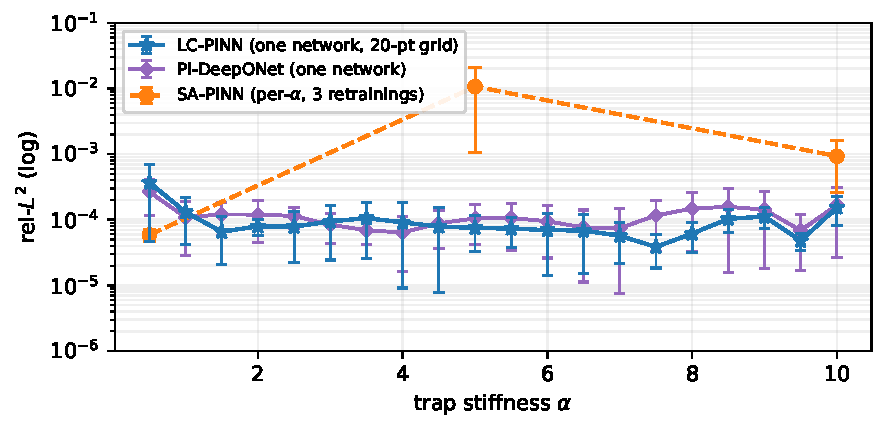
\includegraphics[width=0.75\linewidth]{per_alpha_schrodinger.pdf}
\caption{Per-$\alpha$ rel-$L^2$ on 1D parametric Schrödinger.
LC-PINN (blue, 4 seeds) and PI-DeepONet (purple, 4 seeds) cover the
20-point grid from one trained network each; SA-PINN (orange, 2
seeds) is three separate retrainings at $\alpha\in\{0.5,5.0,10.0\}$.
Error bars are $\pm$std on a log axis.}
\label{fig:per_alpha_schrodinger}
\end{figure}%%%%%%%%%%%%%%%%%%%%%%%%%%%%%%%%%%%%%%%%%%%%%%%%%%%%%%%%%%%%%%%%%%%%%%%%%%%%%%%
%%%%%%%%%%%%%%%%%%%%%%%%%%%%%%%%%%%%%%%%%%%%%%%%%%%%%%%%%%%%%%%%%%%%%%%%%%%%%%%

\end{document}

% This document was modified from the file originally made available by
% Pat Langley and Andrea Danyluk for ICML-2K. This version was created
% by Iain Murray in 2018, and modified by Alexandre Bouchard in
% 2019 and 2021 and by Csaba Szepesvari, Gang Niu and Sivan Sabato in 2022.
% Modified again in 2023 and 2024 by Sivan Sabato and Jonathan Scarlett.
% Previous contributors include Dan Roy, Lise Getoor and Tobias
% Scheffer, which was slightly modified from the 2010 version by
% Thorsten Joachims & Johannes Fuernkranz, slightly modified from the
% 2009 version by Kiri Wagstaff and Sam Roweis's 2008 version, which is
% slightly modified from Prasad Tadepalli's 2007 version which is a
% lightly changed version of the previous year's version by Andrew
% Moore, which was in turn edited from those of Kristian Kersting and
% Codrina Lauth. Alex Smola contributed to the algorithmic style files.
